\documentclass[letterpaper]{article} % DO NOT CHANGE THIS
\usepackage{aaai2027}  % DO NOT CHANGE THIS
% The serif, sans-serif, and monospaced fonts are loaded automatically by
% aaai2027.sty (newtxtext, helvet, courier). DO NOT add \usepackage{times},
% \usepackage{helvet}, \usepackage{courier}, or any other font package.
\usepackage[hyphens]{url}  % DO NOT CHANGE THIS
\usepackage{graphicx} % DO NOT CHANGE THIS
\urlstyle{rm} % DO NOT CHANGE THIS
\def\UrlFont{\rm}  % DO NOT CHANGE THIS
\usepackage{natbib}  % DO NOT CHANGE THIS AND DO NOT ADD ANY OPTIONS TO IT
\usepackage{caption} % DO NOT CHANGE THIS AND DO NOT ADD ANY OPTIONS TO IT
\frenchspacing  % DO NOT CHANGE THIS

% Recommended for better-looking tables
\usepackage{booktabs}
\usepackage{multirow}
\usepackage{amsmath}
\usepackage{amssymb}

%
% Keep the \pdfinfo as shown here. There's no need
% for you to add the /Title and /Author tags.
\pdfinfo{
/TemplateVersion (2027.2)
}

% DISALLOWED PACKAGES
% \usepackage{authblk} -- This package is specifically forbidden
% \usepackage{balance} -- This package is specifically forbidden
% \usepackage{CJK} -- This package is specifically forbidden
% \usepackage{float} -- This package is specifically forbidden
% \usepackage{flushend} -- This package is specifically forbidden
% \usepackage{fullpage} -- This package is specifically forbidden
% \usepackage{geometry} -- This package is specifically forbidden
% \usepackage{hyperref} -- This package is specifically forbidden
% \usepackage{navigator} -- This package is specifically forbidden
% (or any other package that embeds links such as navigator or hyperref)
% \usepackage{indentfirst} -- This package is specifically forbidden
% \usepackage{layout} -- This package is specifically forbidden
% \usepackage{multicol} -- This package is specifically forbidden
% \usepackage{nameref} -- This package is specifically forbidden
% \usepackage{savetrees} -- This package is specifically forbidden
% \usepackage{setspace} -- This package is specifically forbidden
% \usepackage{stfloats} -- This package is specifically forbidden
% \usepackage{tabu} -- This package is specifically forbidden
% \usepackage{titlesec} -- This package is specifically forbidden
% \usepackage{tocbibind} -- This package is specifically forbidden
% \usepackage{ulem} -- This package is specifically forbidden
% \usepackage{wrapfig} -- This package is specifically forbidden
% DISALLOWED COMMANDS
% \nocopyright -- Your paper will not be published if you use this command
% \addtolength -- This command may not be used
% \balance -- This command may not be used
% \baselinestretch -- Your paper will not be published if you use this command
% \clearpage -- No page breaks of any kind may be used for the final version of your paper
% \columnsep -- This command may not be used
% \newpage -- No page breaks of any kind may be used for the final version of your paper
% \pagebreak -- No page breaks of any kind may be used for the final version of your paper
% \pagestyle -- This command may not be used
% \tiny -- This is not an acceptable font size.
% \vspace{- -- No negative value may be used in proximity of a caption, figure, table, section, subsection, subsubsection, or reference
% \vskip{- -- No negative value may be used to alter spacing above or below a caption, figure, table, section, subsection, subsubsection, or reference

\setcounter{secnumdepth}{0} %May be changed to 1 or 2 if section numbers are desired.

\title{CortexDecoder: Image Reconstruction from Cortical Flatmaps}
\author{
    Teo Imoto-Tar\textsuperscript{\rm 1},
    Maxwell Fung\textsuperscript{\rm 2},
    Arnav Gurha\textsuperscript{\rm 1}
}
\affiliations{
    \textsuperscript{\rm 1}University of California, San Diego\\
    \textsuperscript{\rm 2}University of California, Berkeley\\
    timototar@ucsd.edu, maxwellfung@berkeley.edu, agurha@ucsd.edu
}

\begin{document}

\maketitle

\begin{abstract}
Recent brain decoding work has shown the potential of Vision Transformers (ViTs) to learn mappings from neural representations to visual features. Here we present CortexDecoder, a framework that reconstructs viewed images from functional magnetic resonance imaging (fMRI) flatmaps: neural responses projected onto the cortical surface and unfolded into 2D images. We show that (1) a frozen, pretrained cortical foundation model is sufficient for competitive reconstruction, and (2) the model benefits from context across the entire cortex, removing the need for a task-specific region-of-interest (ROI) mask. A frozen CortexMAE encoder turns flatmap patches into brain tokens, and two lightweight cross-attention bridges map these tokens to semantic CLIP embeddings and low-level image features. A frozen SDXL-unCLIP model then generates the final image from the low-level reconstruction, conditioned on the predicted CLIP embedding. On Natural Scenes Dataset (NSD) Subject 1, CortexDecoder is competitive with prior methods while training only about 83M parameters. Code is available at https://github.com/teooi/CortexDecoder.
\end{abstract}

% Uncomment the following to link to your code, datasets, an extended version or similar.
% You must keep this block between (not within) the abstract and the main body of the paper.
% \begin{links}
%     \link{Code}{https://aaai.org/example/code}
% \end{links}

%-------------------------------------------------------------------------
\section{Introduction}
\label{sec:intro}

\begin{figure*}[t]
    \centering
    \includegraphics[width=0.9\textwidth]{Figures/title5.png}
    \caption{Stimuli (top) and CortexDecoder reconstructions (bottom). Images from COCO \cite{lin2015microsoftcococommonobjects} (CC BY 4.0).}
    \label{fig:title}
\end{figure*}

Reconstructing visual experiences from non-invasive functional magnetic resonance imaging (fMRI) remains a central challenge in computational neuroscience. It also has applications in Brain-Computer Interfaces (BCIs), such as communication aids. With the availability of large, open-source fMRI-image datasets like the Natural Scenes Dataset (NSD) \cite{Allen2022Massive7TfMRI}, fMRI has become a natural choice for studying visual decoding. The NSD provides paired fMRI responses together with natural images viewed by subjects, with repeated presentations of visual stimuli across trials. Each sample contains a cortical response corresponding to a viewed image, providing both neural and visual representations for learning fMRI-to-image mappings.

Our central question is: how much information about visual stimuli can we decode from 2D cortical flatmaps? Most brain decoding frameworks follow one of two practices. Some approaches regress directly from raw 3D functional volumes, but this is challenging due to their high dimensionality, noisy voxel-wise signal, and computational cost. Alternatively, conventional approaches that flatten voxel responses into feature vectors or average responses over anatomical parcellations do not explicitly preserve spatial information. This motivated us to explore 2D flatmaps, which preserve cortical geometry while also being directly compatible with modern vision architectures.



We introduce CortexDecoder, a framework that decodes 2D cortical flatmaps into image stimuli using vision transformer (ViT) \cite{dosovitskiy2021imageworth16x16words} models. Since flatmaps are inherently 2D images, we can partition neural activity into discrete patches. We use a frozen pretrained CortexMAE \cite{lane2026scalingvisiontransformersfunctional} encoder---an fMRI foundation model developed by MedARC using the masked autoencoder framework trained on cortical flatmaps. From this encoder, we extract spatially organized brain tokens. By utilizing the full sequence of spatially organized patch tokens from CortexMAE, our architecture preserves local cortical geometry and avoids collapsing the brain representation into a rigid 1D feature vector.

Our cross-attention bridge follows DETR (DEtection TRansformer) \cite{DBLP:journals/corr/abs-2005-12872} and Brain-IT \cite{beliy2025brainitimagereconstructionfmri}, uses learned query vectors to map neural representations to visual feature spaces. Our cross-attention bridge is split into two modules to separately handle predicting semantic and structural visual information. The semantic branch predicts unpooled image CLIP \cite{radford2021learningtransferablevisualmodels} embeddings
which capture the concepts in the scene. whereas the low-level branch targets early visual features such as basic shapes and colors. Many decoding models struggle with low-level visual fidelity, often generating images that match semantically but are unfaithful in terms of pixel correlation and structural similarity. Incorporating a low-level branch targets this gap by providing structural guidance. Finally, we employ MindEye2's \cite{scotti2024mindeye2sharedsubjectmodelsenable} frozen SDXL-unCLIP model \cite{podell2023sdxlimprovinglatentdiffusion} to condition on both the low-level reconstruction and a semantic embedding to produce the final image.

Our main contributions are as follows: (1) we propose CortexDecoder, a novel architecture that uses 2D cortical flatmaps as input for fMRI-to-image reconstruction; (2) we show that flatmaps preserve enough signal for reconstruction, achieving competitive benchmark results; and (3) we show that flatmaps allow for clean tokenization and are compatible with Vision Transformers out of the box.

Our main contributions are as follows: (1) we propose CortexDecoder, a reconstruction framework for cortical flatmap decoding which reads the full sequence of flatmap patch tokens with learned-query cross-attention; (2) we show that our model benefits from context across the entire cortex rather than relying on ROIs; and finally (3) we show that a trained lightweight bridge together with pretrained frozen foundation models is sufficient to achieve performance competitive with other fMRI-to-image decoding models.

%-------------------------------------------------------------------------
\section{Related Work}
\label{sec:related_works}

\subsection{fMRI-to-Image Reconstruction}
Recent methods for fMRI-to-image reconstruction predict the embeddings of pretrained vision models such as CLIP from fMRI and generate images with pretrained diffusion models. Notably, MindEye \cite{scotti2023reconstructingmindseyefmritoimage} predicts CLIP embeddings from fMRI and uses diffusion-based image generation to reconstruct seen images, while Brain-Diffuser \cite{ozcelik2023brain} combines visual representations with latent diffusion. MindEye2 further improves reconstruction through shared-subject training and predicts OpenCLIP ViT-bigG/14 representations \cite{schuhmann2022laionb, ilharco_gabriel_2021_5143773} for SDXL-based image generation. Brain-IT \cite{beliy2025brainitimagereconstructionfmri} maps brain features to image features with a transformer that uses learned queries, a design our bridges follow. Overall, these approaches demonstrate the importance of pretrained generative models for fMRI-to-image reconstruction. However, most of them learn a mapping from voxels with a visual region of interest (ROI), such as NSD's nsdgeneral mask. NeuroPictor \cite{huo2024neuropictorrefiningfmritoimagereconstruction} instead uses cortical flatmaps, but it fine-tunes both its pretrained fMRI encoder and the diffusion model. Our work asks whether these steps are necessary: whether a frozen cortical foundation model, applied to the whole cortex and paired with a frozen generator, is sufficient for competitive reconstruction.

\subsection{fMRI Representations}
How fMRI activity is represented is a central consideration in developing generalizable neural representations. Traditional approaches reduce fMRI volumes with anatomical parcellations, producing compact feature vectors at the expense of spatial information. On the other hand, volumetric representations retain spatial structure but at a substantially greater computational cost. Recent fMRI foundation models have explored self-supervised learning to obtain general-purpose representations from large-scale datasets. For example, BrainLM \cite{Caro2023.09.12.557460} and BrainJEPA \cite{dong2024brainjepabraindynamicsfoundation}, among others, demonstrate the potential of pretrained models for downstream fMRI tasks. CortexMAE \cite{lane2026scalingvisiontransformersfunctional} frames cortical flatmaps as intermediate representations between parcellation and volumetric fMRI, converting cortical activity into 2D maps. These representations benefit from being directly compatible with Vision Transformer architectures. We use a frozen, pretrained CortexMAE encoder to turn each flatmap into a sequence of patch tokens, which our model maps to image features for reconstruction.


\subsection{Semantic and Low-Level Visual Features}
Faithful visual reconstruction benefits from both high-level semantic information and lower-level visual structure. CLIP and OpenCLIP provide semantic visual representations that have been widely adopted for image generation and brain decoding. At the same time, convolutional feature representations such as VGG \cite{simonyan2015deepconvolutionalnetworkslargescale} retain spatial information that may be lost in semantic embeddings. Recent brain decoding approaches have consequently explored multiple visual representations. MindEye and Brain-IT use semantic representations alongside lower-level visual features to improve image reconstruction. CortexDecoder follows this general pipeline by learning separate mappings from brain representations to OpenCLIP semantic tokens and VGG features, which are subsequently combined during image generation.

\begin{figure*}[t]
\centering
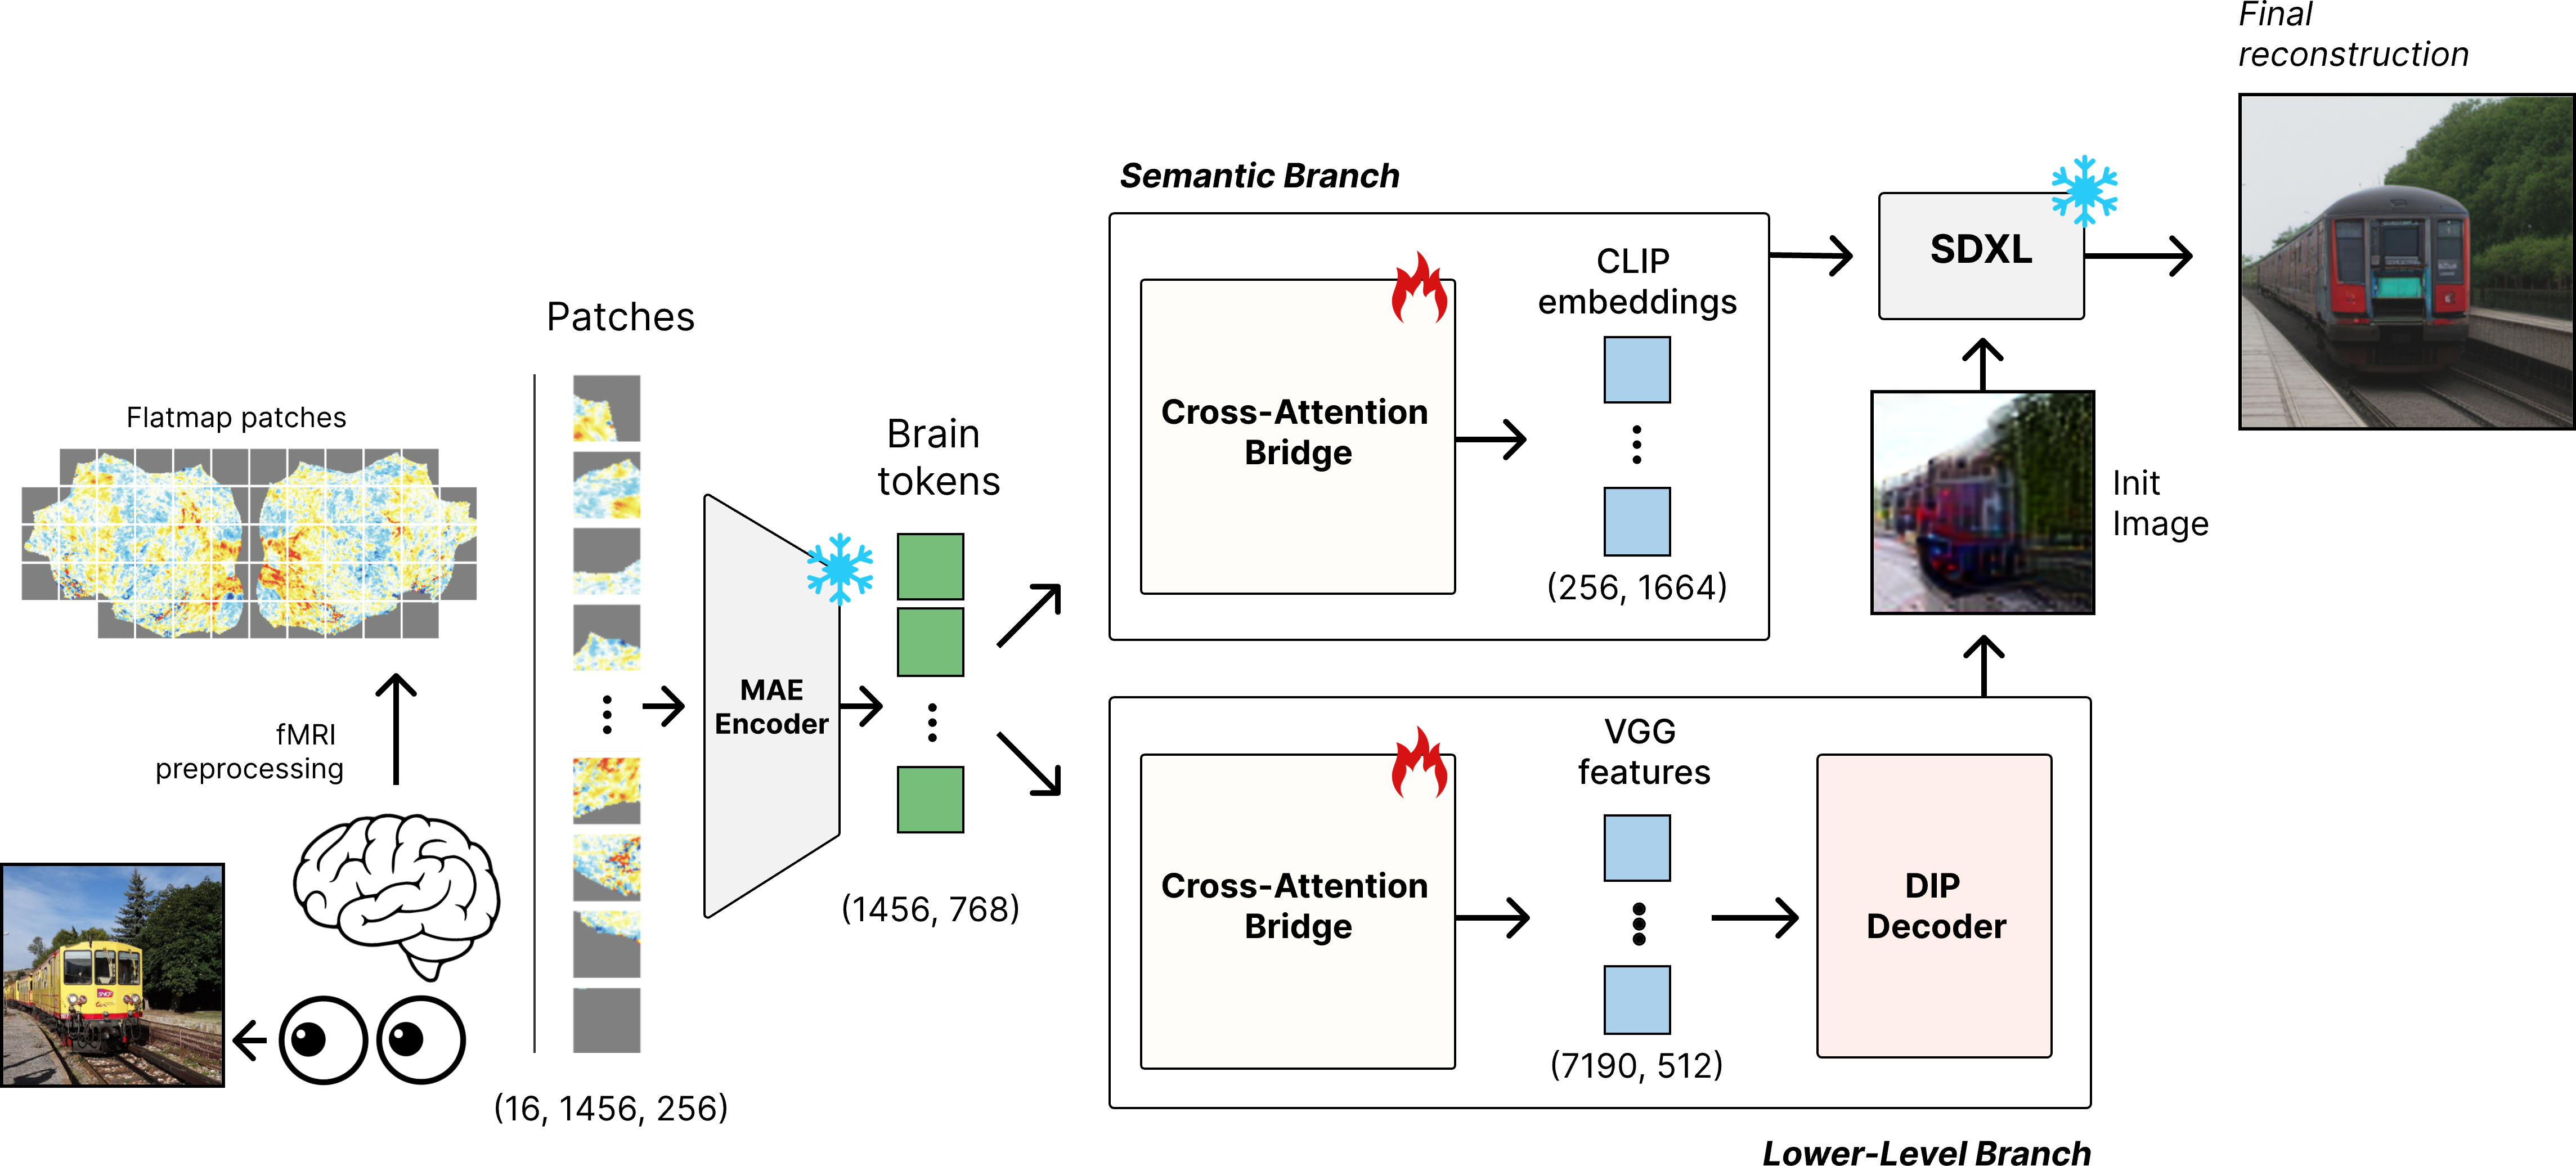
\includegraphics[width=0.75\textwidth]{Figures/model4.png}
\caption{CortexDecoder overview. A frozen CortexMAE encoder turns cortical flatmap patches into 1456 brain tokens. Two cross-attention bridges, the only trained components, predict OpenCLIP tokens (semantic) and VGG16-BN features (low-level). A DIP-inverted low-level image initializes SDXL-unCLIP, which is conditioned on the predicted OpenCLIP tokens to produce the final image. Images from COCO \cite{lin2015microsoftcococommonobjects} (CC BY 4.0).}
\label{fig:model_schematic}
\end{figure*}

%-------------------------------------------------------------------------
\section{CortexDecoder}
\label{sec:cortex_decoder}
CortexDecoder is a two-branch brain decoding framework that maps cortical flatmap representations to high-level semantic and low-level visual features for image reconstruction. The model first encodes cortical flatmaps using a pretrained CortexMAE encoder, producing spatially organized brain tokens. These brain tokens are then fed into the cross-attention bridge, which predicts visual image features. The semantic branch predicts unpooled CLIP embeddings, while the low-level branch predicts VGG features. Finally, the predicted visual representations are provided to a frozen diffusion decoder to reconstruct the corresponding image.

All model training and evaluations were performed on a single NVIDIA H100 GPU (80 GB of vRAM). Both branches were trained separately with AdamW \cite{loshchilov2019decoupledweightdecayregularization} (learning rate 5e-4, weight decay 1e-2) and a batch size of 128 under bfloat16 mixed precision. Both the semantic branch and the low-level branch were trained for 25 epochs. Deep Image Prior inversion at inference uses 2,000 Adam steps per image with 36 images optimized in parallel on the GPU.

\subsection{Natural Scenes Dataset}
The Natural Scenes Dataset (NSD) is a large-scale 7T fMRI dataset in which eight participants viewed natural images drawn from MS-COCO (Microsoft Common Objects in Context) \cite{lin2015microsoftcococommonobjects} across up to 40 scan sessions each. Each session comprises 750 trials; in each trial, one image is presented for 3 seconds, followed by a 1-second blank. Each subject viewed 10,000 unique images, each repeated 3 times, for a total of 30,000 trials per subject. A subset of 1000 images (shared1000) was presented to all subjects and is reserved as a standard test set throughout the literature.

The NSD experiment uses a rapid event-related design in which a new image stimulus is presented every 4 seconds, so successive stimuli occur within the timescale of the hemodynamic response. Because the responses to successive trials overlap, single-trial responses cannot be read directly from the time series. A general linear model (GLM) \cite{10.7554/eLife.77599} performs this deconvolution, and its output is a static spatial map of cortical activity per trial rather than a time series. This is precisely the form that 2D flatmap representations and patch-based tokenization assume. We note that the CortexMAE encoder is spatiotemporal and retains a temporal patch dimension from its pretraining on the BOLD time series. However, because our inputs are static single-trial beta maps, we do not utilize this temporal dimension in CortexDecoder.

\subsection{MAE Encoder and Tokenization}
NSD's surface betas are distributed on a fsaverage mesh \cite{FISCHL2012774} (163,842 vertices per hemisphere). We resample them to fsLR-32k (32,492 vertices per hemisphere, 64,984 total), the standard HCP (Human Connectome Project) \cite{VanEssen_Smith_Barch_Behrens_Yacoub_Ugurbil_2013} mesh on which CortexMAE was pretrained. A pycortex-based \cite{DBLP:journals/fini/GaoHLG15} flat-surface resampler then projects these vertices onto a single-channel $224\times560$ raster, producing the 2D cortical flatmap. Since the projection is defined by a common template mesh rather than by individual anatomy, a given location in the raster corresponds to approximately the same piece of cortex across subjects.

The flatmap is divided into non-overlapping $16\times16$ spatial patches, forming a $14\times35$ grid of 490 cells. Since the cortical surface occupies only part of the bounding box, 364 cells contain cortex and the remaining cells are background. CortexMAE uses a validity mask to exclude these background patches, so only 364 cortical patches are embedded.

CortexMAE is a spatiotemporal masked autoencoder \cite{he2021maskedautoencodersscalablevision} pretrained on BOLD time series. In other words, its patch embedding operates over both space and time. In our case, the input is a single-trial beta map, which has no temporal component. To use the pretrained model, we represent each beta map as a static 16-frame clip. Since we use the CortexMAE encoder out of the box, we also retain its output shape, a sequence of 1456 tokens each with a dimension of 768.

\begin{figure}[t]
\centering
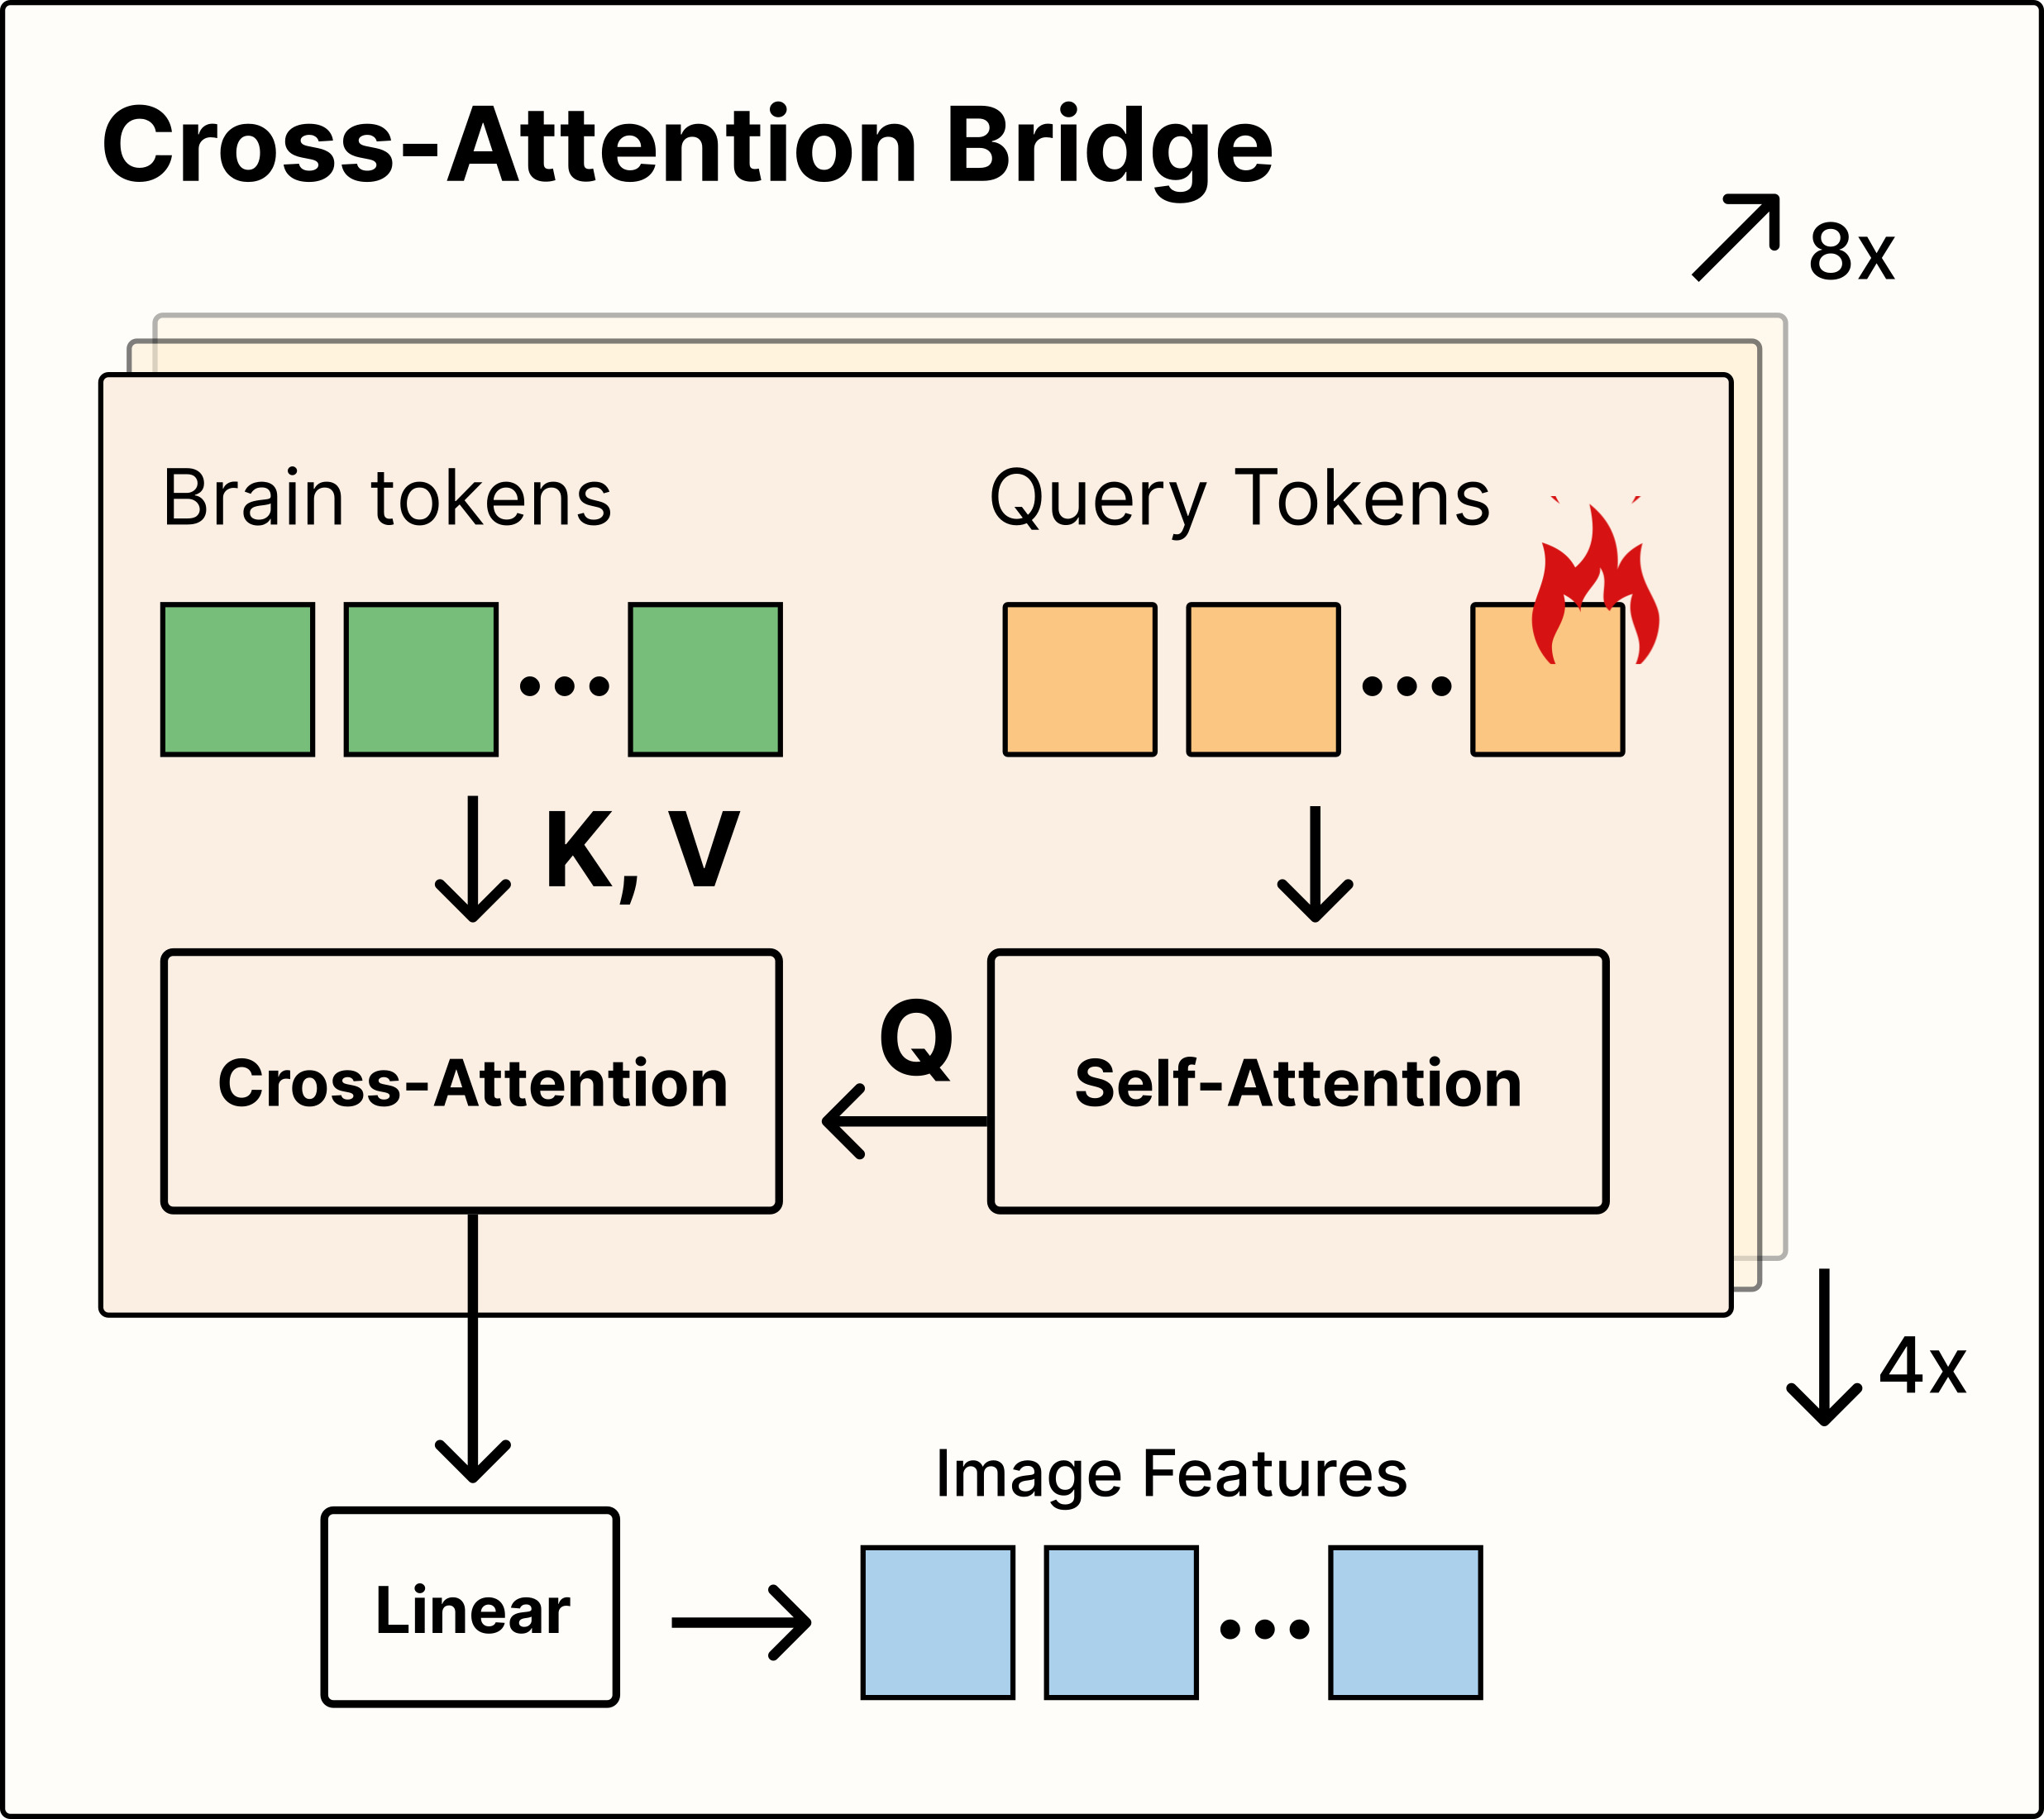
\includegraphics[width=0.8\columnwidth]{Figures/cross.jpg}
\caption{Cross-attention bridge. Learned queries, one per output token, attend to the brain tokens through 4 blocks of self-attention, cross-attention and FFN. A linear layer projects each query to the target feature dimension. Each branch has its own bridge. Images from COCO \cite{lin2015microsoftcococommonobjects} (CC BY 4.0).}
\label{fig:cross_attention_bridge}
\end{figure}

\subsection{Cross-Attention Bridge}
The bridge maps the sequence of brain tokens to a sequence of visual feature tokens. Its design follows DETR (DEtection TRansformer) \cite{DBLP:journals/corr/abs-2005-12872}. We define a set of learned query vectors with one query per output token. These are randomly initialized and trained jointly with the rest of the model. Each query is responsible for predicting one token of the target visual representation.

The brain tokens serve as memory. They are layer-normalized and projected to the model width when the two dimensions differ. In our case, the CortexMAE embedding dimension and the bridge width are both 768, so no projection is needed. The queries are then passed through a stack of transformer decoder layers. Each layer applies self-attention among the queries, then cross-attention from the queries into the brain memory, and finally a position-wise feed-forward network (FFN). Self-attention lets the queries coordinate with one another so that neighboring output tokens can share information. Cross-attention is where the decoding happens. Each query attends over all 1456 brain tokens and pools the ones that carry information about its target feature. A final linear layer projects each decoded query to the dimensionality of the target representation.

We use 4 decoder layers and 8 attention heads. The model width is 768, with a feed-forward dimension of 3072 and dropout of 0.1. The semantic and low-level branches share these settings.

The key property of this design is that the brain representation remains a sequence throughout the pipeline. Each query attends over the full set of brain tokens. A pooled brain vector would make every query attend to the same input and reduce the decoder to a multilayer perceptron (MLP) applied identically at each output position.

We instantiate the bridge twice with one instance per branch and train the two independently rather than sharing a trunk. The semantic branch uses 256 queries and projects to 1664 dimensions. This matches the shape of the unpooled OpenCLIP ViT-bigG/14 \cite{radford2021learningtransferablevisualmodels, ilharco_gabriel_2021_5143773, schuhmann2022laionb} patch tokens that the diffusion decoder expects as conditioning. The low-level branch uses 7190 queries and projects to 512 dimensions. This matches the concatenated token count of the five VGG16-BN feature layers described in the Low-Level Branch section. The two branches therefore differ by more than an order of magnitude in output length. They also optimize different losses, since the semantic target is dense and continuous, while the low-level target is better matched by a contrastive objective.

\begin{equation}
\mathcal{L}_{\mathrm{CLIP}} = \mathrm{MSE}\big(\hat{\mathbf{C}}, \mathbf{C}\big),
\end{equation}

\medskip

where $\hat{\mathbf{C}}, \mathbf{C} \in \mathbb{R}^{256 \times 1664}$ are the predicted and target OpenCLIP token sequences, and the error is averaged over all tokens, dimensions and images in the batch.

To train the low-level branch, we extract target tokens from five intermediate layers of a frozen VGG16-BN network (\texttt{relu1\_2} through \texttt{relu5\_3}, totaling $7{,}190$ spatial tokens of dimension $D=512$). For memory efficiency during training, we randomly sub-sample $K\in \{512, 512, 128, 64, 16\}$ query positions per layer at each step and compute a symmetric position-wise InfoNCE contrastive loss across the mini-batch of $B$ trials:
\begin{equation}
\mathcal{L}_{\mathrm{VGG}} =
\frac{1}{2K}\sum_{k=1}^{K}\left[\mathrm{CE}\!\left({\scriptstyle
\frac{\hat{\mathbf{z}}_{:,k}\mathbf{z}_{:,k}^{\top}}{\tau}},
\mathbf{y}\right) + \mathrm{CE}\!\left({\scriptstyle \frac{\mathbf{z}_{:,
k}\hat{\mathbf{z}}_{:,k}^{\top}}{\tau}}, \mathbf{y}\right)\right],
\end{equation}
where $\hat{\mathbf{z}}_{:,k}, \mathbf{z}_{:,k} \in \mathbb{R}^{B \times
D}$ denote the $\ell_2$-normalized predicted and ground-truth feature
matrices at spatial token $k$, $\tau = 0.07$ is the temperature
hyperparameter, and $\mathbf{y} = (1, \dots, B)^{\top}$ indexes the
matching trial pairs across the batch. The final low-level objective
averages $\mathcal{L}_{\mathrm{VGG}}$ equally across all five VGG16-BN layers.

\subsection{Semantic Branch}
The semantic branch predicts the image representations that condition the diffusion decoder. Its target is the unpooled patch-token sequence produced by the OpenCLIP ViT-bigG/14 vision encoder pretrained on LAION-2B \cite{schuhmann2022laionb}. For each stimulus image, we take the 256 patch tokens before the final projection and discard the class (CLS) token. Each token is 1664-dimensional. The bridge therefore uses 256 queries and projects to 1664 dimensions so that its output matches the target.

We use an unpooled token sequence rather than a single pooled embedding. A pooled CLIP vector summarizes an image but discards its spatial layout. A token sequence retains that layout and gives the diffusion decoder a spatially structured conditioning signal. The diffusion decoder we use is a pretrained SDXL-unCLIP model whose cross-attention was trained to condition on exactly 256 bigG tokens of 1664 dimensions. Matching this shape means the decoder can be used frozen with no fine-tuning on our part. Predicting a smaller CLIP variant would require retraining the decoder's conditioning pathway.

The OpenCLIP encoder is frozen and used only to produce targets. We extract the token sequence for every stimulus image once and cache it. During training, the branch never runs the image encoder. The branch is trained with mean squared error between the predicted and target token sequences, averaged over all 256 positions and 1664 dimensions.

\begin{figure}[t]
\centering
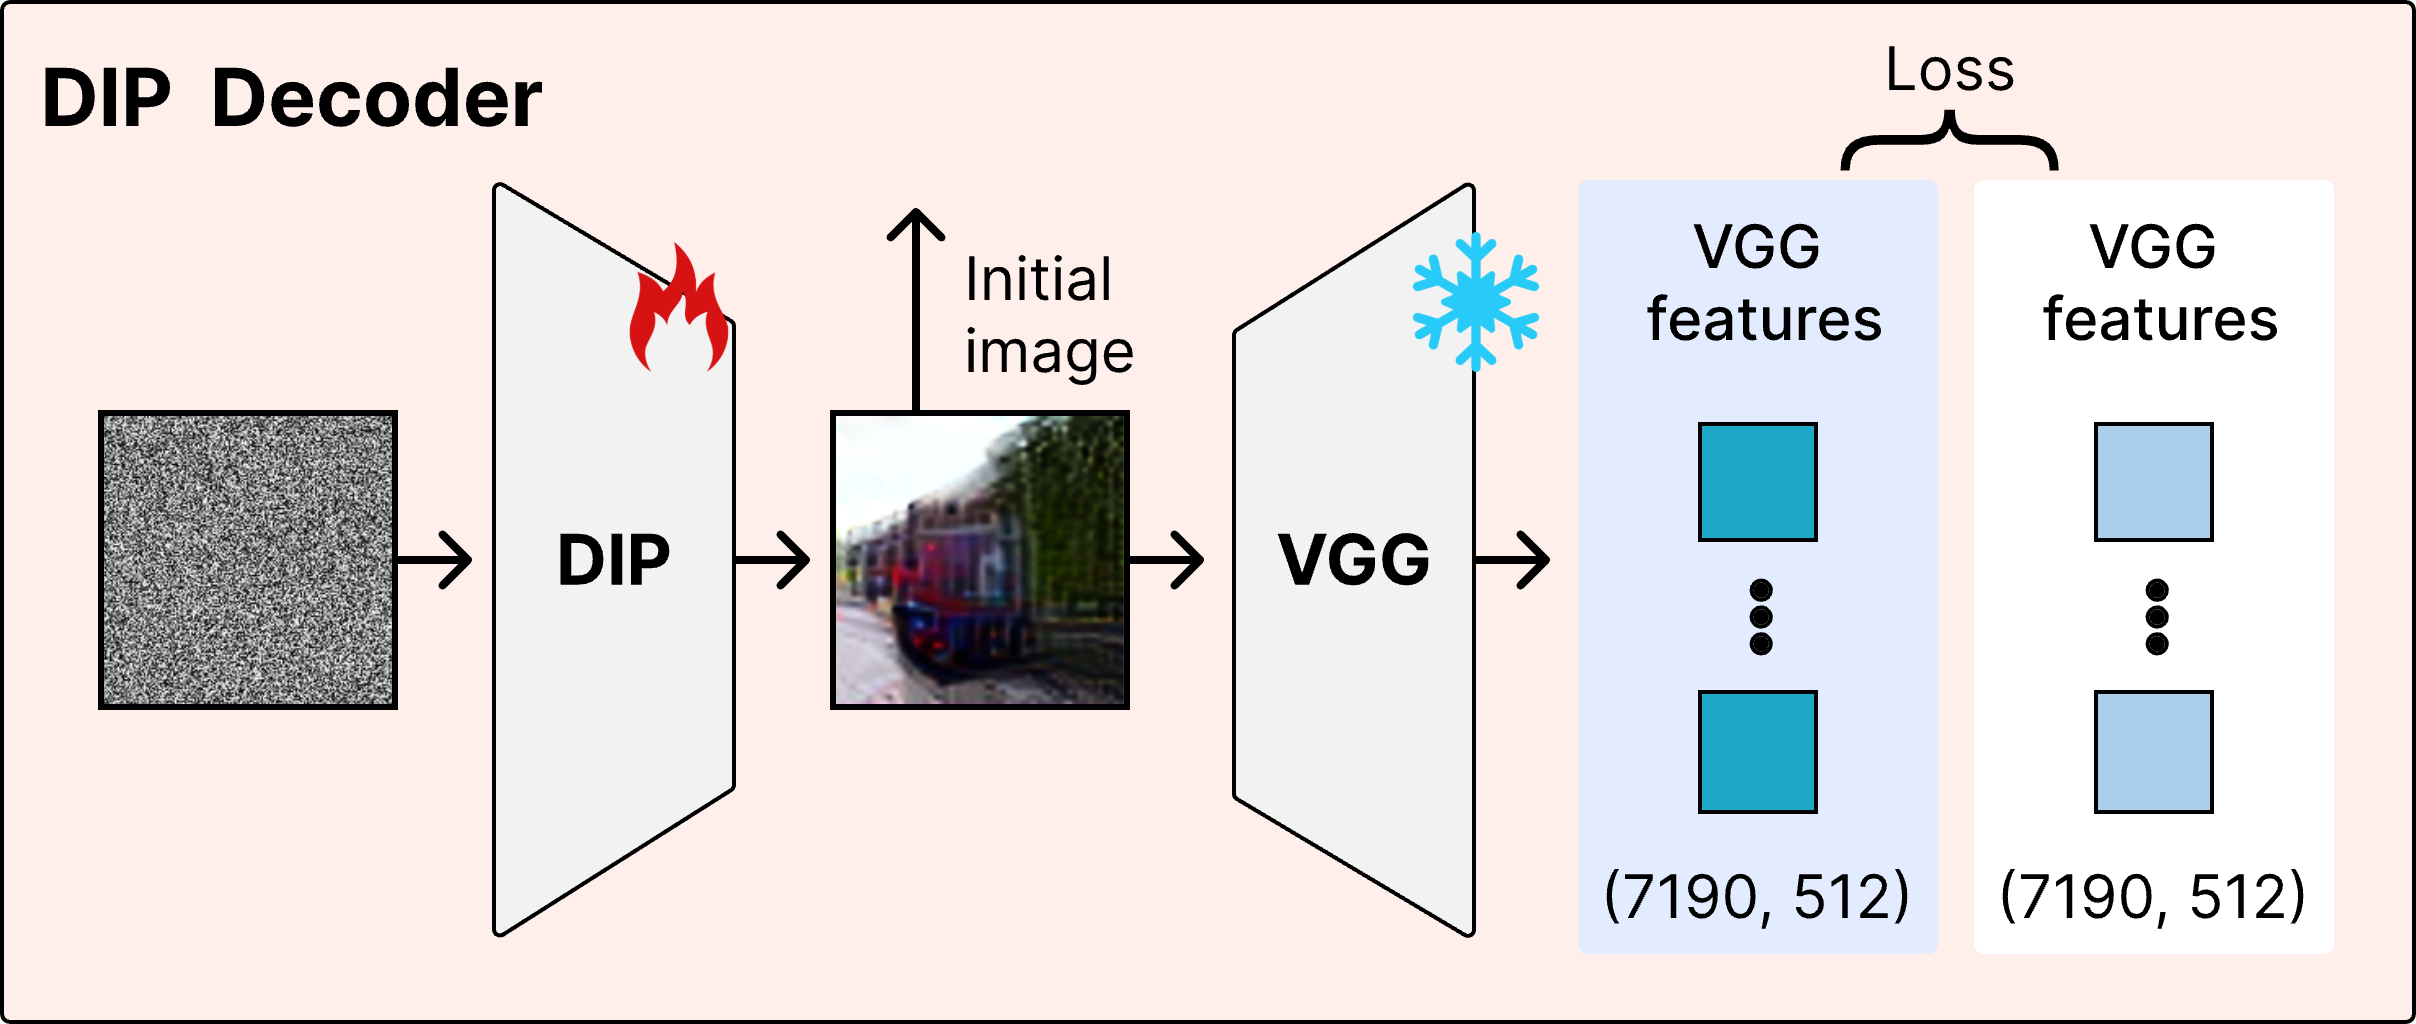
\includegraphics[width=0.95\columnwidth]{Figures/DIP3.png}
\caption{Low-level reconstruction with Deep Image Prior. A U-Net maps noise to an image whose frozen VGG16-BN features are matched to the bridge's predicted features. After 2000 optimization steps, its output is the low-level reconstruction.}
\label{fig:dip_reconstruction}
\end{figure}

\subsection{Low-Level Branch}
\label{sec:low_level}
From the predicted VGG feature representation, we reconstruct a low-level image through Deep Image Prior (DIP) inversion. The VGG representation consists of the stacked outputs of five convolutional layers of the VGG16-BN image model.

To convert this representation into the initial image, we optimize a separate DIP U-Net for each image. The U-Net is a small encoder-decoder convolutional generator that maps random Gaussian noise to an RGB image, which is then passed through a frozen VGG16-BN network. The extracted VGG features are compared against the brain-predicted VGG representation using an MSE loss. The gradient is backpropagated only through the DIP U-Net, iteratively updating the generator for a fixed 2000 optimization steps to produce the final low-level reconstruction.

\subsection{Final Image Reconstruction}
To generate the final image reconstruction, we combine the image capturing low-level features generated using DIP with the semantic CLIP prediction using the MindEye2 Stable Diffusion XL unCLIP model (SDXL-unCLIP). SDXL-unCLIP is a pretrained image generation model that generates images from OpenCLIP ViT-bigG/14 image embeddings instead of text-prompt embeddings. The intention is for the low-level DIP image to provide layout, color, and coarse structure while the predicted OpenCLIP ViT-bigG/14 tokens contribute the semantic context of the image.

We first add Gaussian noise to the low-level image to partially corrupt fine detail while preserving coarse layout and color. This re-noised image becomes the initial state for SDXL-unCLIP, anchoring the image structure. The predicted OpenCLIP token representation then steers the denoising process toward the correct semantic context, turning the blurry low-level reconstruction into a detailed final image. With this approach, the reconstruction should reflect both the content and the structure of the stimulus. We run this diffusion process multiple times for each image and select the reconstruction whose downscaled version has the lowest MSE relative to the low-level reconstruction. This keeps the final image from straying too far from the predicted low-level image structure.

\begin{figure}[t]
\centering
\includegraphics[width=0.75\columnwidth]{Figures/stacked_triptych_collage4.png}
\caption{Stimulus (left), low-level DIP reconstruction (middle) and final diffusion reconstruction (right). Images from COCO \cite{lin2015microsoftcococommonobjects} (CC BY 4.0).}
\label{fig:stacked_triptych}
\end{figure}

%-------------------------------------------------------------------------
\section{Results}
\label{sec:results}

\begin{table*}[t]
\centering
\small
\setlength{\tabcolsep}{3pt}
\begin{tabular*}{\textwidth}{@{\extracolsep{\fill}}llcccccccc@{}}
\toprule
& & \multicolumn{4}{c}{Low-Level} & \multicolumn{4}{c}{High-Level} \\
\cmidrule(lr){3-6}\cmidrule(lr){7-10}
\textbf{Method} & \textbf{Input}
& PixCorr$\uparrow$ & SSIM$\uparrow$ & Alex(2)$\uparrow$ & Alex(5)$\uparrow$
& Incep$\uparrow$ & CLIP$\uparrow$ & Eff$\downarrow$ & SwAV$\downarrow$ \\
\midrule
Brain-Diffuser \cite{ozcelik2023brain} & Voxels
& 0.305 & 0.367 & 96.7\% & 97.4\%
& 87.8\% & 92.5\% & 0.768 & 0.415 \\
MindEye1$^\ast$ \cite{scotti2023reconstructingmindseyefmritoimage} & Voxels
& \textbf{0.390} & 0.337 & 97.4\% & 98.7\%
& 94.5\% & \textbf{94.6\%} & 0.630 & 0.358 \\
MindEye2$^\dagger$ \cite{scotti2024mindeye2sharedsubjectmodelsenable} & Voxels
& 0.374 & \textbf{0.439} & 97.8\% & \underline{99.1\%}
& \textbf{96.2\%} & 93.6\% & \textbf{0.609} & \underline{0.338} \\
NeuroPictor$^\dagger$ \cite{huo2024neuropictorrefiningfmritoimagereconstruction} & Flatmap
& 0.277 & 0.385 & \textbf{98.8\%} & \textbf{99.3\%}
& \textbf{96.2\%} & \underline{94.5\%} & \underline{0.619} & \textbf{0.334} \\
\textbf{CortexDecoder (ours)}$^\ast$ & Flatmap
& \underline{0.377} & \underline{0.417} & \underline{97.9\%} & 99.0\%
& \underline{94.9\%} & 93.2\% & 0.640 & 0.372 \\
\midrule
\textbf{CortexDecoder (low-level)} & Flatmap
& 0.390 & 0.407 & 97.6\% & 99.2\%
& 90.9\% & 75.9\% & 0.845 & 0.580 \\
\bottomrule
\end{tabular*}
\caption{Quantitative comparison of CortexDecoder and prior methods on NSD Subject 1. Baseline results are taken from each paper. The last row is our low-level image before diffusion. \textbf{Bold}: best; \underline{underline}: second best. $^\dagger$Pretrained on multiple subjects. $^\ast$Best of several diffusion samples (MindEye1: 16; ours: 10).}
\label{tab:reconstruction}
\end{table*}

We evaluate CortexDecoder on the NSD shared1000 test set, which is kept completely separate from the training and validation data to prevent leakage. All metrics compare reconstructions against the stimulus images viewed by each subject, and we report the average over Subjects 1 and 2. We report PixCorr (Pixel Correlation), SSIM (Structural Similarity Index Measure) \cite{1284395}, AlexNet(2), AlexNet(5) \cite{NIPS2012_c399862d}, InceptionV3 \cite{szegedy2015rethinkinginceptionarchitecturecomputer}, CLIP \cite{radford2021learningtransferablevisualmodels}, EfficientNet-B1 \cite{tan2020efficientnetrethinkingmodelscaling} and SwAV-ResNet50 \cite{caron2021unsupervisedlearningvisualfeatures}. PixCorr and SSIM measure pixel and structural similarity while AlexNet, InceptionV3 and CLIP measure feature-space similarity. EfficientNet and SwAV report correlation distance, where lower is better.

We report metrics for both the low-level DIP reconstruction and the final diffusion reconstruction. This allows us to evaluate the contribution of the low-level branch separately from the semantic conditioning. Because diffusion is stochastic, we generate ten candidates per image. Then we select the generated image with the lowest pixelwise MSE to the low-level reconstruction after resizing. This approach does not use ground-truth images and favors candidates that preserve the predicted structure.

\subsection{Reconstruction Benchmarks}
CortexDecoder is competitive with prior methods in capturing low-level and mid-level features in reconstructed images. Specifically, our model performs well on PixCorr and SSIM, reflecting the contribution of the low-level branch. However, it is weaker at capturing semantic features in the reconstructed images.

The results show that introducing semantic conditioning degrades low-level fidelity. For example, the low-level reconstruction on its own scores higher on most low-level metrics (PixCorr, AlexNet(2) and AlexNet(5)) than the final reconstruction, where semantic conditioning is introduced in the diffusion stage. We conclude that the final reconstruction, which combines semantic and low-level representations, improves on semantic metrics at the expense of low-level performance.

% TODO (AAAI workshop): single-subject (Subj 1) comparison against per-subject numbers from prior work.
% TODO: Ablations -- (a) bridge depth / transformer block count, (b) number of MHA heads/layers,
%       (c) semantic-branch losses (e.g., MSE vs. cosine vs. contrastive vs. combinations).
% \subsection{Ablation Studies}

%-------------------------------------------------------------------------
\section{Conclusion}
\label{sec:conclusion}
We introduce CortexDecoder, an fMRI-to-image reconstruction framework that uses 2D cortical flatmaps as neural representations for visual decoding. By converting cortical flatmaps into patch tokens, CortexDecoder enables the use of Vision Transformers while preserving the spatial structure of cortical responses. A pretrained CortexMAE encoder produces brain tokens, which are then mapped through two cross-attention branches: one for semantic features and one for low-level image reconstruction. These predictions are then passed to a fine-tuned SDXL-unCLIP image generation model, which takes the predicted low-level image as its initial image and generates the final reconstruction conditioned on the predicted semantic embedding.

Our results show that cortical flatmaps preserve enough information to support brain decoding. CortexDecoder is strongest at low-level reconstruction, particularly on the PixCorr and SSIM metrics, across the two subjects we evaluated. Overall, flatmaps are a promising fMRI representation for brain decoding, as we have demonstrated for image reconstruction.

\section{Limitations}
\label{sec:limitations}
Due to compute and budget constraints, our experiments are limited to NSD Subjects 1 and 2, instead of the full four-subject evaluation used in the prior works discussed above. Our results in Table~\ref{tab:reconstruction} are therefore averaged over two subjects, while the baselines are averaged over four, so the comparison is not strictly like-for-like. A clear direction for future work is to extend our method to all four subjects and evaluate whether the observed patterns hold across them.

Additionally, our compute and budget constraints restricted hyperparameter tuning, design iteration, and the repeated full evaluations that would have helped optimize our metrics. We were only able to perform one full evaluation run, rather than multiple design iterations, which may partially explain the gap to other state-of-the-art models on the high-level metrics.

\section{Future Work}
\label{sec:future_work}
In future work, we will extend our experiments from NSD Subjects 1 and 2 to the full four-subject setting used by other papers. This would evaluate whether the observed performance of our pipeline holds up across subjects with differing brain anatomies.

We would likely implement this by introducing a functional clustering space shared across subjects. Specifically, we would summarize each flatmap patch across trials into a single descriptor vector, then fit a Gaussian Mixture Model \cite{dempster1977maximum} to map brain patches from all subjects into a common cluster space. A cross-attention layer could then compress the patches assigned to each cluster into a fixed set of cluster tokens. Similar strategies have proven effective in prior work for training a single transferable model across many subjects \cite{beliy2026wisdomcrowdbrainsuniversal, beliy2025brainitimagereconstructionfmri}.

Together, these extensions would enable a more direct comparison against prior multi-subject methods and test whether our approach remains competitive at scale.

Another direction is to replace CLIP as the target semantic representation with the embedding space of a more recent model such as SigLIP2 \cite{tschannen2025siglip2multilingualvisionlanguage}. One limitation of our current pipeline is that semantic conditioning on CLIP embeddings comes at the expense of low-level performance. Replacing CLIP with a stronger semantic embedding model such as SigLIP2 could improve visual-semantic alignment and, in turn, performance on both low-level and high-level evaluations. This may require training an SDXL decoder that accepts SigLIP2 embeddings as conditioning inputs.

\begin{figure}[t]
\centering
\includegraphics[width=0.9\columnwidth]{Figures/comparison_boxed_labeled.png}
\caption{Stimulus, CortexDecoder, MindEye2 and NeuroPictor reconstructions (left to right). Images from COCO \cite{lin2015microsoftcococommonobjects} (CC BY 4.0).}
\label{fig:comparison}
\end{figure}

\bibliography{references}

% Check whether the conference requires a reproducibility checklist to be included in the paper.
% If so, you can uncomment the following line and ajust the path to include it.
% \makeatletter
\@ifundefined{isChecklistMainFile}{
  % We are compiling a standalone document
  \newif\ifreproStandalone
  \reproStandalonetrue
}{
  % We are being \input into the main paper
  \newif\ifreproStandalone
  \reproStandalonefalse
}
\makeatother

\ifreproStandalone
\documentclass[letterpaper]{article}
\usepackage[submission]{aaai2027}
\setlength{\pdfpagewidth}{8.5in}
\setlength{\pdfpageheight}{11in}
\frenchspacing

\begin{document}
\fi
\setlength{\leftmargini}{20pt}
\makeatletter\def\@listi{\leftmargin\leftmargini \topsep .5em \parsep .5em \itemsep .5em}
\def\@listii{\leftmargin\leftmarginii \labelwidth\leftmarginii \advance\labelwidth-\labelsep \topsep .4em \parsep .4em \itemsep .4em}
\def\@listiii{\leftmargin\leftmarginiii \labelwidth\leftmarginiii \advance\labelwidth-\labelsep \topsep .4em \parsep .4em \itemsep .4em}\makeatother

\setcounter{secnumdepth}{0}
\renewcommand\thesubsection{\arabic{subsection}}
\renewcommand\labelenumi{\thesubsection.\arabic{enumi}}

\newcounter{checksubsection}
\newcounter{checkitem}[checksubsection]

\newcommand{\checksubsection}[1]{%
  \refstepcounter{checksubsection}%
  \paragraph{\arabic{checksubsection}. #1}%
  \setcounter{checkitem}{0}%
}

\newcommand{\checkitem}{%
  \refstepcounter{checkitem}%
  \item[\arabic{checksubsection}.\arabic{checkitem}.]%
}
\newcommand{\question}[2]{\normalcolor\checkitem #1 #2 \color{blue}}
\newcommand{\ifyespoints}[1]{\makebox[0pt][l]{\hspace{-15pt}\normalcolor #1}}

\section*{Reproducibility Checklist}

\vspace{1em}
\hrule
\vspace{1em}

\textbf{Instructions for Authors:}

This document outlines key aspects for assessing reproducibility. Please provide your input by editing this \texttt{.tex} file directly.

For each question (that applies), replace the ``Type your response here'' text with your answer.

\vspace{1em}
\noindent
\textbf{Example:} If a question appears as
%
\begin{center}
\noindent
\begin{minipage}{.9\linewidth}
\ttfamily\raggedright
\string\question \{Proofs of all novel claims are included\} \{(yes/partial/no)\} \\
Type your response here
\end{minipage}
\end{center}
you would change it to:
\begin{center}
\noindent
\begin{minipage}{.9\linewidth}
\ttfamily\raggedright
\string\question \{Proofs of all novel claims are included\} \{(yes/partial/no)\} \\
yes
\end{minipage}
\end{center}
%
Please make sure to:
\begin{itemize}\setlength{\itemsep}{.1em}
\item Replace ONLY the ``Type your response here'' text and nothing else.
\item Use one of the options listed for that question (e.g., \textbf{yes}, \textbf{no}, \textbf{partial}, or \textbf{NA}).
\item \textbf{Not} modify any other part of the \texttt{\string\question} command or any other lines in this document.\\
\end{itemize}

You can \texttt{\string\input} this .tex file right before \texttt{\string\end\{document\}} of your main file or compile it as a stand-alone document. Check the instructions on your conference's website to see if you will be asked to provide this checklist with your paper or separately.

\vspace{1em}
\hrule
\vspace{1em}

% The questions start here

\checksubsection{General Paper Structure}
\begin{itemize}

\question{Includes a conceptual outline and/or pseudocode description of AI methods introduced}{(yes/partial/no/NA)}
Type your response here

\question{Clearly delineates statements that are opinions, hypothesis, and speculation from objective facts and results}{(yes/no)}
Type your response here

\question{Provides well-marked pedagogical references for less-familiar readers to gain background necessary to replicate the paper}{(yes/no)}
Type your response here

\end{itemize}
\checksubsection{Theoretical Contributions}
\begin{itemize}

\question{Does this paper make theoretical contributions?}{(yes/no)}
Type your response here

	\ifyespoints{\vspace{1.2em}If yes, please address the following points:}
        \begin{itemize}

	\question{All assumptions and restrictions are stated clearly and formally}{(yes/partial/no)}
	Type your response here

	\question{All novel claims are stated formally (e.g., in theorem statements)}{(yes/partial/no)}
	Type your response here

	\question{Proofs of all novel claims are included}{(yes/partial/no)}
	Type your response here

	\question{Proof sketches or intuitions are given for complex and/or novel results}{(yes/partial/no)}
	Type your response here

	\question{Appropriate citations to theoretical tools used are given}{(yes/partial/no)}
	Type your response here

	\question{All theoretical claims are demonstrated empirically to hold}{(yes/partial/no/NA)}
	Type your response here

	\question{All experimental code used to eliminate or disprove claims is included}{(yes/no/NA)}
	Type your response here

	\end{itemize}
\end{itemize}

\checksubsection{Dataset Usage}
\begin{itemize}

\question{Does this paper rely on one or more datasets?}{(yes/no)}
Type your response here

\ifyespoints{If yes, please address the following points:}
\begin{itemize}

	\question{A motivation is given for why the experiments are conducted on the selected datasets}{(yes/partial/no/NA)}
	Type your response here

	\question{All novel datasets introduced in this paper are included in a data appendix}{(yes/partial/no/NA)}
	Type your response here

	\question{All novel datasets introduced in this paper will be made publicly available upon publication of the paper with a license that allows free usage for research purposes}{(yes/partial/no/NA)}
	Type your response here

	\question{All datasets drawn from the existing literature (potentially including authors' own previously published work) are accompanied by appropriate citations}{(yes/no/NA)}
	Type your response here

	\question{All datasets drawn from the existing literature (potentially including authors' own previously published work) are publicly available}{(yes/partial/no/NA)}
	Type your response here

	\question{All datasets that are not publicly available are described in detail, with explanation why publicly available alternatives are not scientifically satisficing}{(yes/partial/no/NA)}
	Type your response here

\end{itemize}
\end{itemize}

\checksubsection{Computational Experiments}
\begin{itemize}

\question{Does this paper include computational experiments?}{(yes/no)}
Type your response here

\ifyespoints{If yes, please address the following points:}
\begin{itemize}

	\question{This paper states the number and range of values tried per (hyper-) parameter during development of the paper, along with the criterion used for selecting the final parameter setting}{(yes/partial/no/NA)}
	Type your response here

	\question{Any code required for pre-processing data is included in the appendix}{(yes/partial/no)}
	Type your response here

	\question{All source code required for conducting and analyzing the experiments is included in a code appendix}{(yes/partial/no)}
	Type your response here

	\question{All source code required for conducting and analyzing the experiments will be made publicly available upon publication of the paper with a license that allows free usage for research purposes}{(yes/partial/no)}
	Type your response here

	\question{All source code implementing new methods have comments detailing the implementation, with references to the paper where each step comes from}{(yes/partial/no)}
	Type your response here

	\question{If an algorithm depends on randomness, then the method used for setting seeds is described in a way sufficient to allow replication of results}{(yes/partial/no/NA)}
	Type your response here

	\question{This paper specifies the computing infrastructure used for running experiments (hardware and software), including GPU/CPU models; amount of memory; operating system; names and versions of relevant software libraries and frameworks}{(yes/partial/no)}
	Type your response here

	\question{This paper formally describes evaluation metrics used and explains the motivation for choosing these metrics}{(yes/partial/no)}
	Type your response here

	\question{This paper states the number of algorithm runs used to compute each reported result}{(yes/no)}
	Type your response here

	\question{Analysis of experiments goes beyond single-dimensional summaries of performance (e.g., average; median) to include measures of variation, confidence, or other distributional information}{(yes/no)}
	Type your response here

	\question{The significance of any improvement or decrease in performance is judged using appropriate statistical tests (e.g., Wilcoxon signed-rank)}{(yes/partial/no)}
	Type your response here

	\question{This paper lists all final (hyper-)parameters used for each model/algorithm in the paper’s experiments}{(yes/partial/no/NA)}
	Type your response here


\end{itemize}
\end{itemize}
\ifreproStandalone
\end{document}
\fi


\end{document}


